\documentclass{standalone}
\usepackage{tikz}
\usetikzlibrary{intersections, calc}
\usepackage{hsbcommon}
\begin{document}
    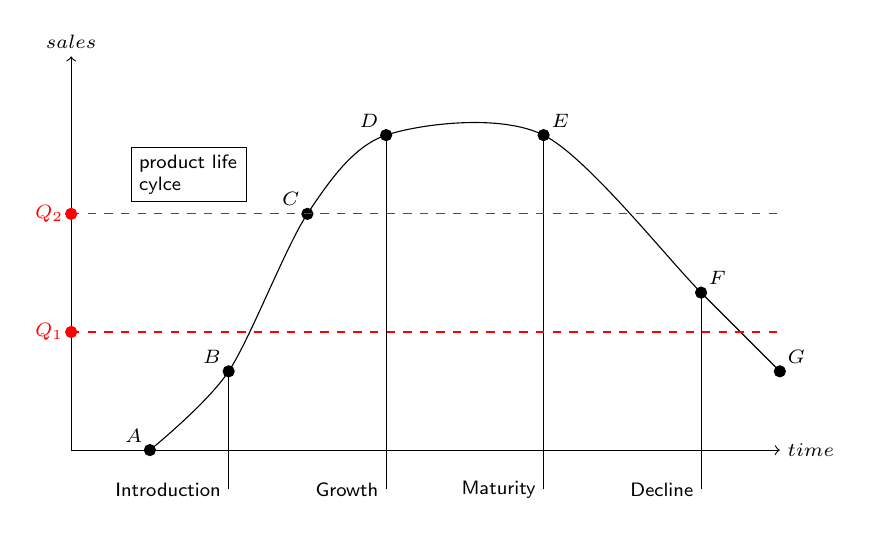
\begin{tikzpicture}[font=\sffamily] \scriptsize
        \draw[->] (0,0) -- (9,0) node[right] (Q) {$time$};
        \draw[->] (0,0) -- (0,5) node[above] (P) {$sales$};

        \coordinate (A) at (1,0); \filldraw (A) circle (2pt) node [above left] {$A$};
        \coordinate (B) at (2,1); \filldraw (B) circle (2pt) node [above left] {$B$};
        \coordinate (C) at (3,3); \filldraw (C) circle (2pt) node [above left] {$C$};
        \coordinate (D) at (4,4); \filldraw (D) circle (2pt) node [above left] {$D$};
        \coordinate (E) at (6,4); \filldraw (E) circle (2pt) node [above right] {$E$};
        \coordinate (F) at (8,2); \filldraw (F) circle (2pt) node [above right] {$F$};
        \coordinate (G) at (9,1); \filldraw (G) circle (2pt) node [above right] {$G$};
 
        \draw [name path=demand] plot [smooth] coordinates {(A) (B) (C) (D) (E)  (F) (G) };
        % \node[above right] at (G) {$turnovers$};

        \draw [name path=eins] (B |-, -0.5) node[left] {Introduction} -- (B);
        \draw [name path=zwei] (D |-, -0.5) node[left] {Growth} -- (D);
        \draw [name path=zwei] (E |-, -0.5) node[left] {Maturity} -- (E);
        \draw [name path=zwei] (F |-, -0.5) node[left] {Decline} -- (F);

        \coordinate (Q) at (0,1.5); \filldraw[red] (Q) circle (2pt) node [left] {$Q_1$}; 
        \draw [red, dashed] (0, |- Q) -- (9, |- Q) ;

        \coordinate (R) at (0,3); \filldraw[red] (R) circle (2pt) node [left] {$Q_2$}; 
        \draw [red, dashed] (0, |- R) -- (9, |- R) ;

        \node[draw, text width=12ex] at (1.5,3.5) {product life cylce};
        
        
    \end{tikzpicture}
\end{document}